\section{含参积分}
\label{sec:integral-parametric}

许多量是“对一个变量积分、随另一个变量变化”的函数。例如$F(t)=\int_0^\infty e^{-tx}\,\mathrm dx$随衰减率$t$变化，模型的平均损失随参数变化。设$(X,\mathcal A,\mu)$是测度空间，$I\subseteq\mathbb R$是区间，$f:I\times X\to\mathbb R$（或$\mathbb C$），并且对每个$t\in I$，截面$f(t,\cdot)$都是可测函数。只要积分有意义，就得到一元函数
\[
 F(t)=\int_Xf(t,x)\,\mathrm d\mu(x),
\]
称为\term{含参积分}（parameter-dependent integral）。测度和积分区域都固定不动，参数的变化完全体现在被积函数上。本节的问题是：$f$对$t$连续或可微时，$F$是否也连续或可微？参数的变化是一种极限过程，因此答案来自第~\ref{sec:integral-limits}节的控制收敛定理；关键是找到对一族参数同时有效的可积控制。

\subsection{积分关于参数的连续性}
\label{sec:integral-parametric-continuity}

对每个固定的$x$，$t\mapsto f(t,x)$连续，只说明每个位置上的取值连续变化。质量却可能随参数移向无穷远或集中到越来越小的区域，这在任何固定位置上都看不出来。用一个可积函数同时控制附近全部参数的被积函数，就排除了这两种可能。

\begin{theorem}[含参积分的连续性]
\label{thm:integral-parametric-continuity}
设$t_0\in I$，$J$是$t_0$在$I$中的一个邻域（相对于$I$），$g\ge0$关于$\mu$可积。若
\begin{enumerate}
 \item 对$\mu$-几乎所有$x$，$t\mapsto f(t,x)$在$t_0$处连续；
 \item 对每个$t\in J$，$|f(t,x)|\le g(x)$对$\mu$-几乎所有$x$成立，
\end{enumerate}
则对$t\in J$，$F(t)$有限，并且$F$在$t_0$处连续。
\end{theorem}

\begin{proof}
由条件(2)，每个$f(t,\cdot)$（$t\in J$）都被可积函数$g$控制，因而可积，$F(t)$有限。任取$J$中的序列$t_n\to t_0$。条件(1)的例外集是一个零测集；条件(2)对每个$t_n$和$t_0$各有一个零测例外集，可数个零测集之并仍零测。在这些例外集之外，$f(t_n,x)\to f(t_0,x)$且$|f(t_n,x)|\le g(x)$，控制收敛定理~\ref{thm:integral-dominated-convergence}给出$F(t_n)\to F(t_0)$。实变量函数的序列判据说明$F$在$t_0$连续。
\end{proof}

证明中合并例外集时只用到了可数个参数值，所以条件(2)的例外集可以随$t$改变；条件(1)的例外集则是对一个固定的$x$集合说的，不随参数变化。控制只需在所考察点的一个邻域内成立，不必用一个函数覆盖整个参数区间。

\begin{example}[局部控制与整体控制]
\label{ex:integral-parametric-local}
令$F(t)=\int_0^\infty e^{-tx}\,\mathrm dx=1/t$（$t>0$）。在$(0,\infty)$上找不到统一的控制：$\sup_{t>0}e^{-tx}=1$，常数$1$在$[0,\infty)$上不可积。但固定$t_0>0$，在邻域$J=(t_0/2,\infty)$上有$e^{-tx}\le e^{-t_0x/2}$，右侧可积，积分为$2/t_0$。定理给出$F$在$t_0$连续；$t_0$任意，所以$F$在整个$(0,\infty)$上连续。每个参数点各用自己的包络就够了。
\end{example}

\paragraph{控制失效的情形}
在参数区间的边界附近，局部控制可能不存在，此时结论也可能失效。在$[0,\infty)$上令$f(t,x)=te^{-tx}$（$t>0$），并按逐点极限补充$f(0,x)=0$。对每个$t>0$，
\[
 F(t)=\int_0^\infty te^{-tx}\,\mathrm dx=1,
\]
而$F(0)=0$，所以$F$在$t=0$处不连续，尽管对每个固定的$x$都有$f(t,x)\to0=f(0,x)$。图~\ref{fig:integral-parameter-continuity}显示了原因：$t$越小，曲线越低越平，同样为$1$的质量被推向越来越远的地方。由$\int_c^\infty te^{-tx}\,\mathrm dx=e^{-tc}$，一半质量位于$x\ge(\ln2)/t$处，这个位置随$t\downarrow0$趋于无穷。

任何控制函数都必须位于这族曲线的上包络之上。对$x>1/\delta$，函数$t\mapsto te^{-tx}$在$t=1/x\in(0,\delta)$处取最大值，所以
\[
 \sup_{0<t<\delta}te^{-tx}=\frac1{ex},
\]
它在$(1/\delta,\infty)$上不可积。于是$t=0$的任何邻域都没有可积控制，定理的条件不成立。这个例子提醒我们，结论只适用于已经核对了控制条件的参数范围。

\begin{figure}[!htbp]
\centering
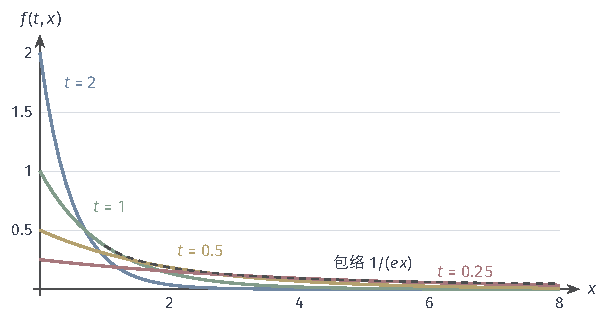
\includegraphics[width=102.807mm]{figures/02-abstract-mathematics/01-metric-and-measure/tikz/c3-parameter-continuity/figure.pdf}
\caption{含参积分中质量的逃逸。四条实线是$f(t,x)=te^{-tx}$在$t=2,1,0.5,0.25$时的图像，每条曲线下的面积都是$1$；$t$越小，质量越向右摊开。虚线是包络$\sup_tte^{-tx}=1/(ex)$（在$t=1/x$处取到，画在$x\ge1$部分），它在无穷远处不可积，所以$t=0$附近没有可积控制。}
\label{fig:integral-parameter-continuity}
\end{figure}

\subsection{积分号下求导}
\label{sec:integral-differentiate-under-sign}

若$f(t,x)$对$t$可微，自然希望$F'(t)=\int_X\partial_tf(t,x)\,\mathrm d\mu(x)$，即总量的变化率等于各处变化率的累计。这种运算称为\term{积分号下求导}（differentiation under the integral sign）。左侧是差商$\bigl(F(t+h)-F(t)\bigr)/h=\int_X\frac{f(t+h,x)-f(t,x)}{h}\,\mathrm d\mu(x)$在$h\to0$时的极限，所以这又是一次极限与积分的交换。控制的对象是差商；对实值函数，中值定理把差商的控制归结为偏导数的控制。

\begin{theorem}[积分号下求导]
\label{thm:integral-differentiate-under-integral}
设$J\subseteq I$是开区间，$f$为实值，$N\in\mathcal A$为$\mu$零测集，$g\ge0$关于$\mu$可积，且
\begin{enumerate}
 \item 对每个$x\notin N$，$t\mapsto f(t,x)$在$J$上可微，并且$|\partial_tf(t,x)|\le g(x)$对所有$t\in J$成立；
 \item 存在$t_1\in J$，使$f(t_1,\cdot)$关于$\mu$可积。
\end{enumerate}
则对每个$t\in J$，$f(t,\cdot)$可积，$F$在$J$上可微，并且
\begin{equation}
 F'(t)=\int_X\partial_tf(t,x)\,\mathrm d\mu(x),
 \label{eq:integral-differentiate-under-integral}
\end{equation}
其中$\partial_tf(t,\cdot)$在$N$上取值$0$。
\end{theorem}

\begin{proof}
对$x\notin N$与$t\in J$，中值定理给出$|f(t,x)-f(t_1,x)|\le|t-t_1|g(x)$，所以$|f(t,\cdot)|\le|f(t_1,\cdot)|+|t-t_1|g$几乎处处成立，右侧可积，$f(t,\cdot)$可积。

固定$t\in J$，任取非零序列$h_n\to0$且$t+h_n\in J$，令
\[
 q_n(x)=\frac{f(t+h_n,x)-f(t,x)}{h_n}.
\]
每个$q_n$是两个可测函数之差的倍数，因而可测。对$x\notin N$，$q_n(x)\to\partial_tf(t,x)$，所以$\partial_tf(t,\cdot)\mathbf 1_{X\setminus N}$是可测函数列$q_n\mathbf 1_{X\setminus N}$的逐点极限，它是可测的；这正是选择在$N$上取零的原因。中值定理又给出$|q_n(x)|\le g(x)$（$x\notin N$）。由控制收敛定理，
\[
 \frac{F(t+h_n)-F(t)}{h_n}=\int_Xq_n\,\mathrm d\mu\longrightarrow\int_X\partial_tf(t,x)\,\mathrm d\mu(x).
\]
序列$h_n$任意，由序列判据，$F$在$t$处可微且导数为式~\eqref{eq:integral-differentiate-under-integral}右侧。
\end{proof}

复值的$f$可以对实部和虚部分别使用定理。条件(1)中的零测集$N$和控制函数$g$都不能随参数改变：参数有不可数多个，各参数的例外集之并未必零测，也未必可测。这一组条件便于核对，但只是充分条件；更一般地，只需在$t$的邻域内用同一个可积函数控制全部差商。

\begin{example}[对$e^{-tx}$在积分号下逐阶求导]
\label{ex:integral-differentiate-exponential}
仍取$F(t)=\int_0^\infty e^{-tx}\,\mathrm dx=1/t$。固定$t_0>0$，取$J=(t_0/2,3t_0/2)$，则对$t\in J$，
\[
 |\partial_te^{-tx}|=xe^{-tx}\le xe^{-t_0x/2},
\]
右侧可积，分部积分得其积分为$4/t_0^2$。条件(2)由$F(t_0)$有限保证，例外集可取$N=\varnothing$。定理给出$F'(t_0)=-\int_0^\infty xe^{-t_0x}\,\mathrm dx$；与直接求导$F'(t_0)=-1/t_0^2$比较，得$\int_0^\infty xe^{-t_0x}\,\mathrm dx=1/t_0^2$。

高阶导数要逐阶重新核对。设已经得到
\[
 F^{(k)}(t)=(-1)^k\int_0^\infty x^ke^{-tx}\,\mathrm dx,
\]
则第$k+1$阶需要的控制是
\[
 |\partial_t(x^ke^{-tx})|=x^{k+1}e^{-tx}\le x^{k+1}e^{-t_0x/2}\qquad(t\in J),
\]
右侧可积，故可再求一次导。逐阶完成后与$\frac{\mathrm d^k}{\mathrm dt^k}t^{-1}=(-1)^kk!\,t^{-k-1}$比较，得到
\[
 \int_0^\infty x^ke^{-tx}\,\mathrm dx=\frac{k!}{t^{k+1}}\qquad(t>0,\ k=0,1,2,\ldots).
\]
每一阶用的都是$t_0$附近的局部控制；若参数范围包含任意接近零的正数，同一个包络就不再适用。
\end{example}

\paragraph{偏导存在不等于可以交换}
偏导数逐点存在并不足以交换求导与积分。对$x\in(0,1)$与$t\ge0$，令$f(t,x)=tx/(x^2+t^2)$（$t>0$），$f(0,x)=0$。在$t=0$处，对每个固定的$x$，差商$f(t,x)/t=x/(x^2+t^2)\to1/x$，所以右偏导数$\partial_tf(0,x)=1/x$处处存在，但$1/x$在$(0,1)$上不可积。另一方面，令$u=x^2+t^2$直接积分，
\[
 F(t)=\frac t2\ln\frac{1+t^2}{t^2}\quad(t>0),\qquad F(0)=0,
\]
所以$F(t)/t=\frac12\ln(1+t^{-2})\to\infty$（$t\downarrow0$），$F$在$0$处没有有限的右导数。差商$x/(x^2+t^2)$在$x=t$处等于$1/(2t)$，峰值随$t\downarrow0$无界地升高并移向原点，找不到统一的可积控制，交换就失效了。
